\documentclass{article}
\usepackage{amsmath,amssymb,amsthm}
\usepackage{enumerate}
\usepackage{mathtools}
\usepackage{graphicx}
\usepackage{caption}
\usepackage{bm}
\newtheorem{theorem}{Theorem}
\newtheorem{question}[theorem]{Question}
\newtheorem{answer}[theorem]{Solution}
\newcommand{\vect}[1]{\boldsymbol{\mathbf{#1}}}
\newcommand{\myvec}[1]{\ensuremath{\begin{pmatrix}#1\end{pmatrix}}}
\begin{document}
\begin{question}
	Show that the vectors $\begin{pmatrix} 
		 +2\\-1\\+1 
	\end{pmatrix}$, $\begin{pmatrix} 
	 +1\\-3\\-5 
\end{pmatrix}$ and $\begin{pmatrix} 
+3\\-4\\-4 
\end{pmatrix}$ form the vertices of a right angled triangle.
\end{question}
Solution. Let $\vect{A}$,$\vect{B}$  and $\vect{C}$ be given vectors such that $\vect{A} =\begin{pmatrix} 
	+2\\-1\\+1 
\end{pmatrix}$,\\     
$\vect{B}= \begin{pmatrix} 
+1\\-3\\-5 
\end{pmatrix}$ and $\vect{C}= \begin{pmatrix} 
+3\\-4\\-4 
\end{pmatrix}$.\\
To show that $\vect{A}$, $\vect{B}$ and $\vect{C}$ form the vertices of a right angled triangle. First we need to show that $\vect{A}$, $\vect{B}$ and $\vect{C}$ are indeed vertices of a triangle.\\
For this we need to see if the vertices satisfy triangle inequality. Let $a$, $b$ and $c$ denote the length of vectors $(\vect{A}- \vect{B})$, $(\vect{B}-\vect{C})$ and $(\vect{C}- \vect{A})$. Now,\\
$a=\sqrt{41}$, $b=\sqrt{6}$ and $c=\sqrt{35}$. We can see that  $a+b>c$, 
$a+c>b$ and $b+c >a$. Thus, the given vectors $\vect{A}$, $\vect{B}$ and $\vect{C}$ form the vertices of a triangle.\\

\begin{figure}[!htb]
	
	\centering
	
	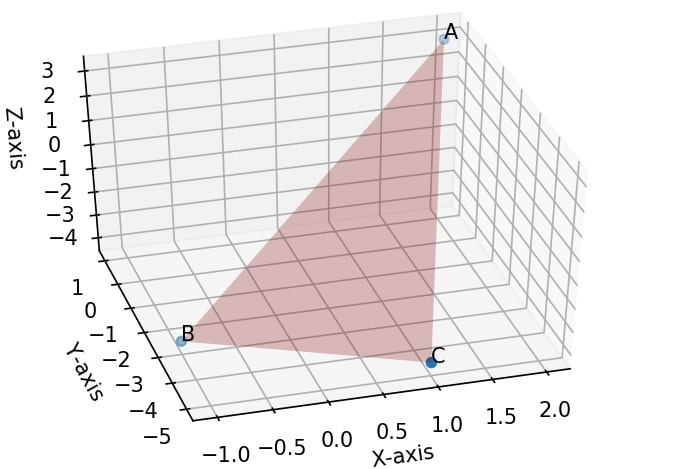
\includegraphics[width=\columnwidth]{assignment1fig-1.jpg}
	
	\caption{\label{fig1}}
	
	\label{fig:}
	
\end{figure}

To prove, the $\triangle ABC$ is a right triangle, we need to calculate the inner product of all the below vectors and check if any one of them is 0.:
\begin{align}
	\langle \vect{A}-\vect{C}   ,\vect{B}-\vect{C}\rangle = (\vect{A} -\vect{C})^T (\vect{B}-\vect{C}) = (-1 \quad+3 \quad +5) \myvec{-2 \\ +1 \\ -1}  = 00 \\
	\langle \vect{A}-\vect{B}   ,\vect{C}-\vect{B}\rangle = (\vect{A} -\vect{B})^T (\vect{C}-\vect{B})
	 = (+1 \quad +2 \quad +6) \myvec{+2 \\ -1 \\ +1} = 06 \\
    \langle \vect{B}-\vect{A}   ,\vect{C}-\vect{A}\rangle = (\vect{B} -\vect{A})^T (\vect{C}-\vect{A}) = (-1\quad-2 \quad-6) \myvec{+1\\-3\\-5} = 35 
\end{align}
Clearly, from ($1$) we can see that $\triangle$ABC is right angled at C.
\end{document}
